\chapter{Introduction}
\chaptermark{Introduction}
\label{chapter:introduction}

\epigraph{\textit{IoT without security means Internet of Threats}}{Stéphane Nappo}

\minitoc

%%%%%%%%%%%%%%%%%%%%%%%%%%%%%%%%%%%%%%%%%%%%%%%%%%%%%%%%%%%%%%%%%%%%%%%%%%%%%%%%%%%%%%%%%%%%%%%
\section{Context}
An embedded system is a specialised computing system designed to perform dedicated functions or tasks within a larger mechanical or electrical system. Unlike general-purpose computers, embedded systems are optimised for specific control operations and are typically integrated into the hardware they manage. These systems are characterised by their compact size, low power consumption, and real-time performance constraints. They consist of microcontrollers or microprocessors, along with memory and input/output interfaces, tailored to meet the precise requirements of the application they serve. Embedded systems are ubiquitous in modern technology, powering a wide range of devices from household appliances and medical equipment to industrial machines and automotive systems, ensuring efficiency, reliability, and functionality in their operations.

\begin{figure}[ht]
    \centering
    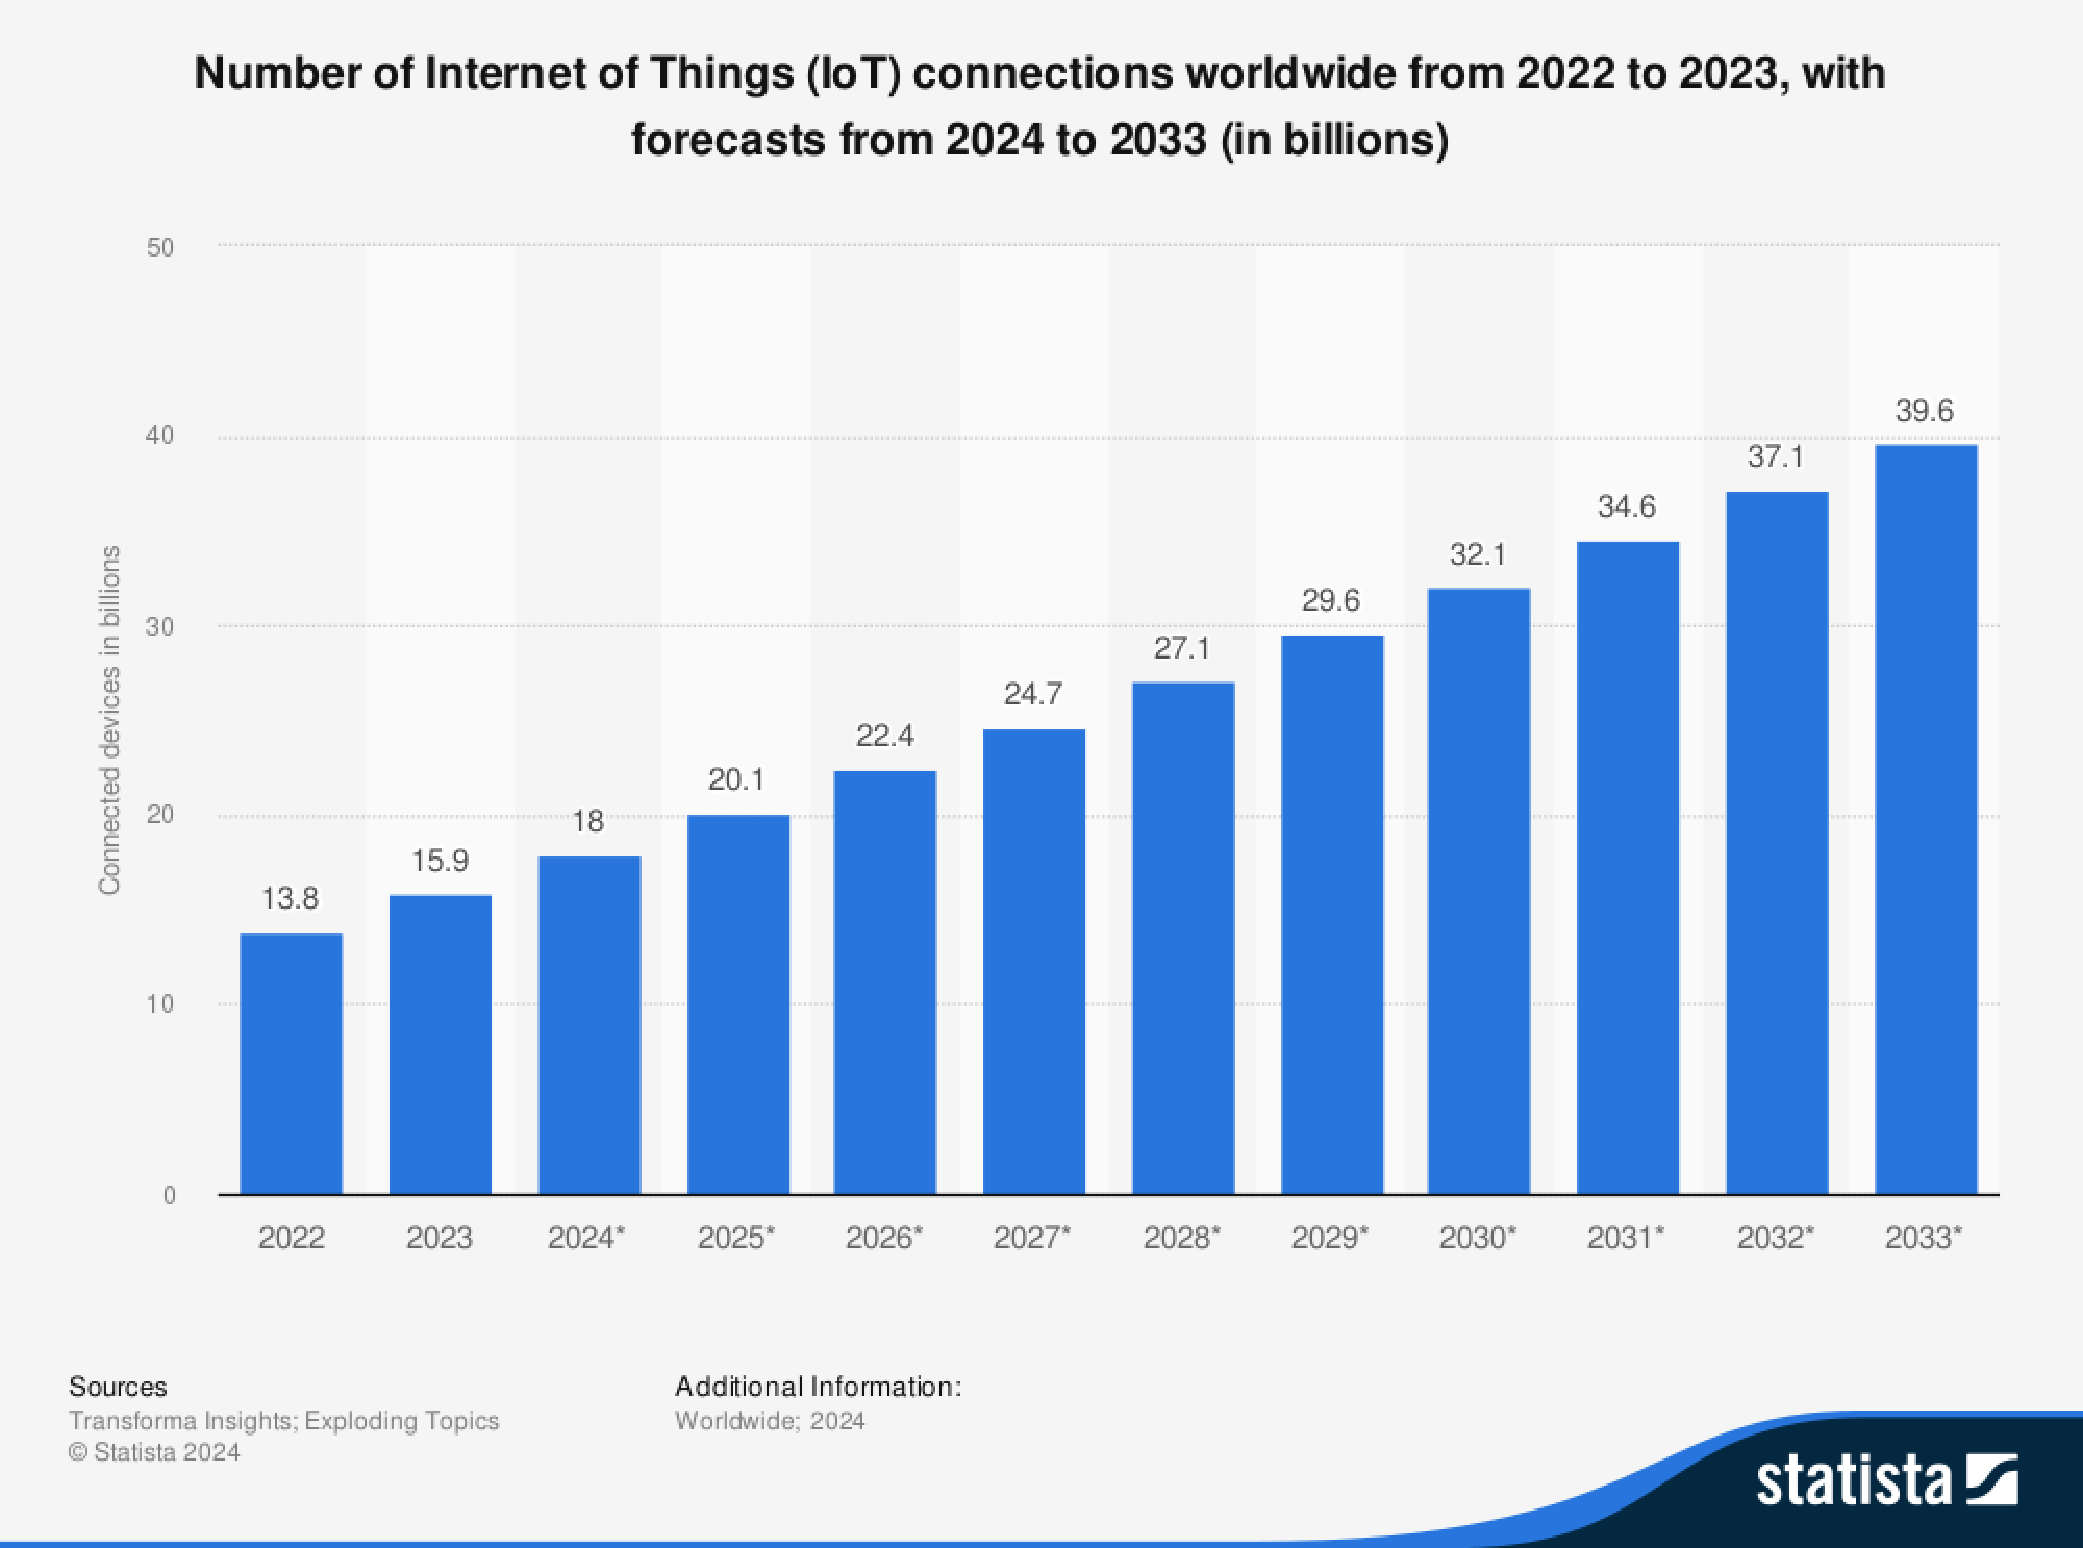
\includegraphics[width=\linewidth, trim={1.25cm 4.75cm 1cm 3.75cm}, clip]{c1_intro/img/iot_forecasts.pdf}
    \caption{Number of IoT devices worldwide 2022-2023, with forecasts to 2033 (from~\cite{statista_iot})}
    \label{fig:iot_forecasts}
\end{figure}

The Internet of Things (IoT) has revolutionised the way we interact with technology, enabling seamless connectivity and communication between a myriad of devices. These devices are part of our daily lives, from the connected light bulb to autonomous cars. These devices collect and share data about how they are used and the environment in which they operate.  Immense amounts of data are also being generated by connected cars, production and transport applications. Today, Industrial IoT (IIoT) data represents the largest and fastest-growing volume.
To do this, they rely on sensors embedded in every physical device, such as mobile phones, smart watches, medical devices (pacemakers, cardiac defibrillators, etc.), but also in recent cars or in agriculture. These sensors generate data that are more or less criticals, but these data exist and they are at the mercy of cyber attacks.
According to forecasts, the number of IoT devices in use worldwide is estimated to reach approximatively 40 billions in 2033~\cite{statista_iot} as shown in Figure~\ref{fig:iot_forecasts}, while, today, in 2024, we are around 18 billions. The economic impact of IoT is substantial, with worldwide consumer IoT revenue expected to rise from \$181.5 billion in 2020 to 621.6 billion euros by 2030~\cite{statista_iot_revenu} as shown in Figure~\ref{fig:iot_revenue}.
As IoT continues to expand its reach, the importance of ensuring robust software security in these systems becomes increasingly critical. IoT devices, often characterised by limited resources and large-scale deployment, present unique security and privacy challenges.

\begin{figure}[ht]
    \centering
    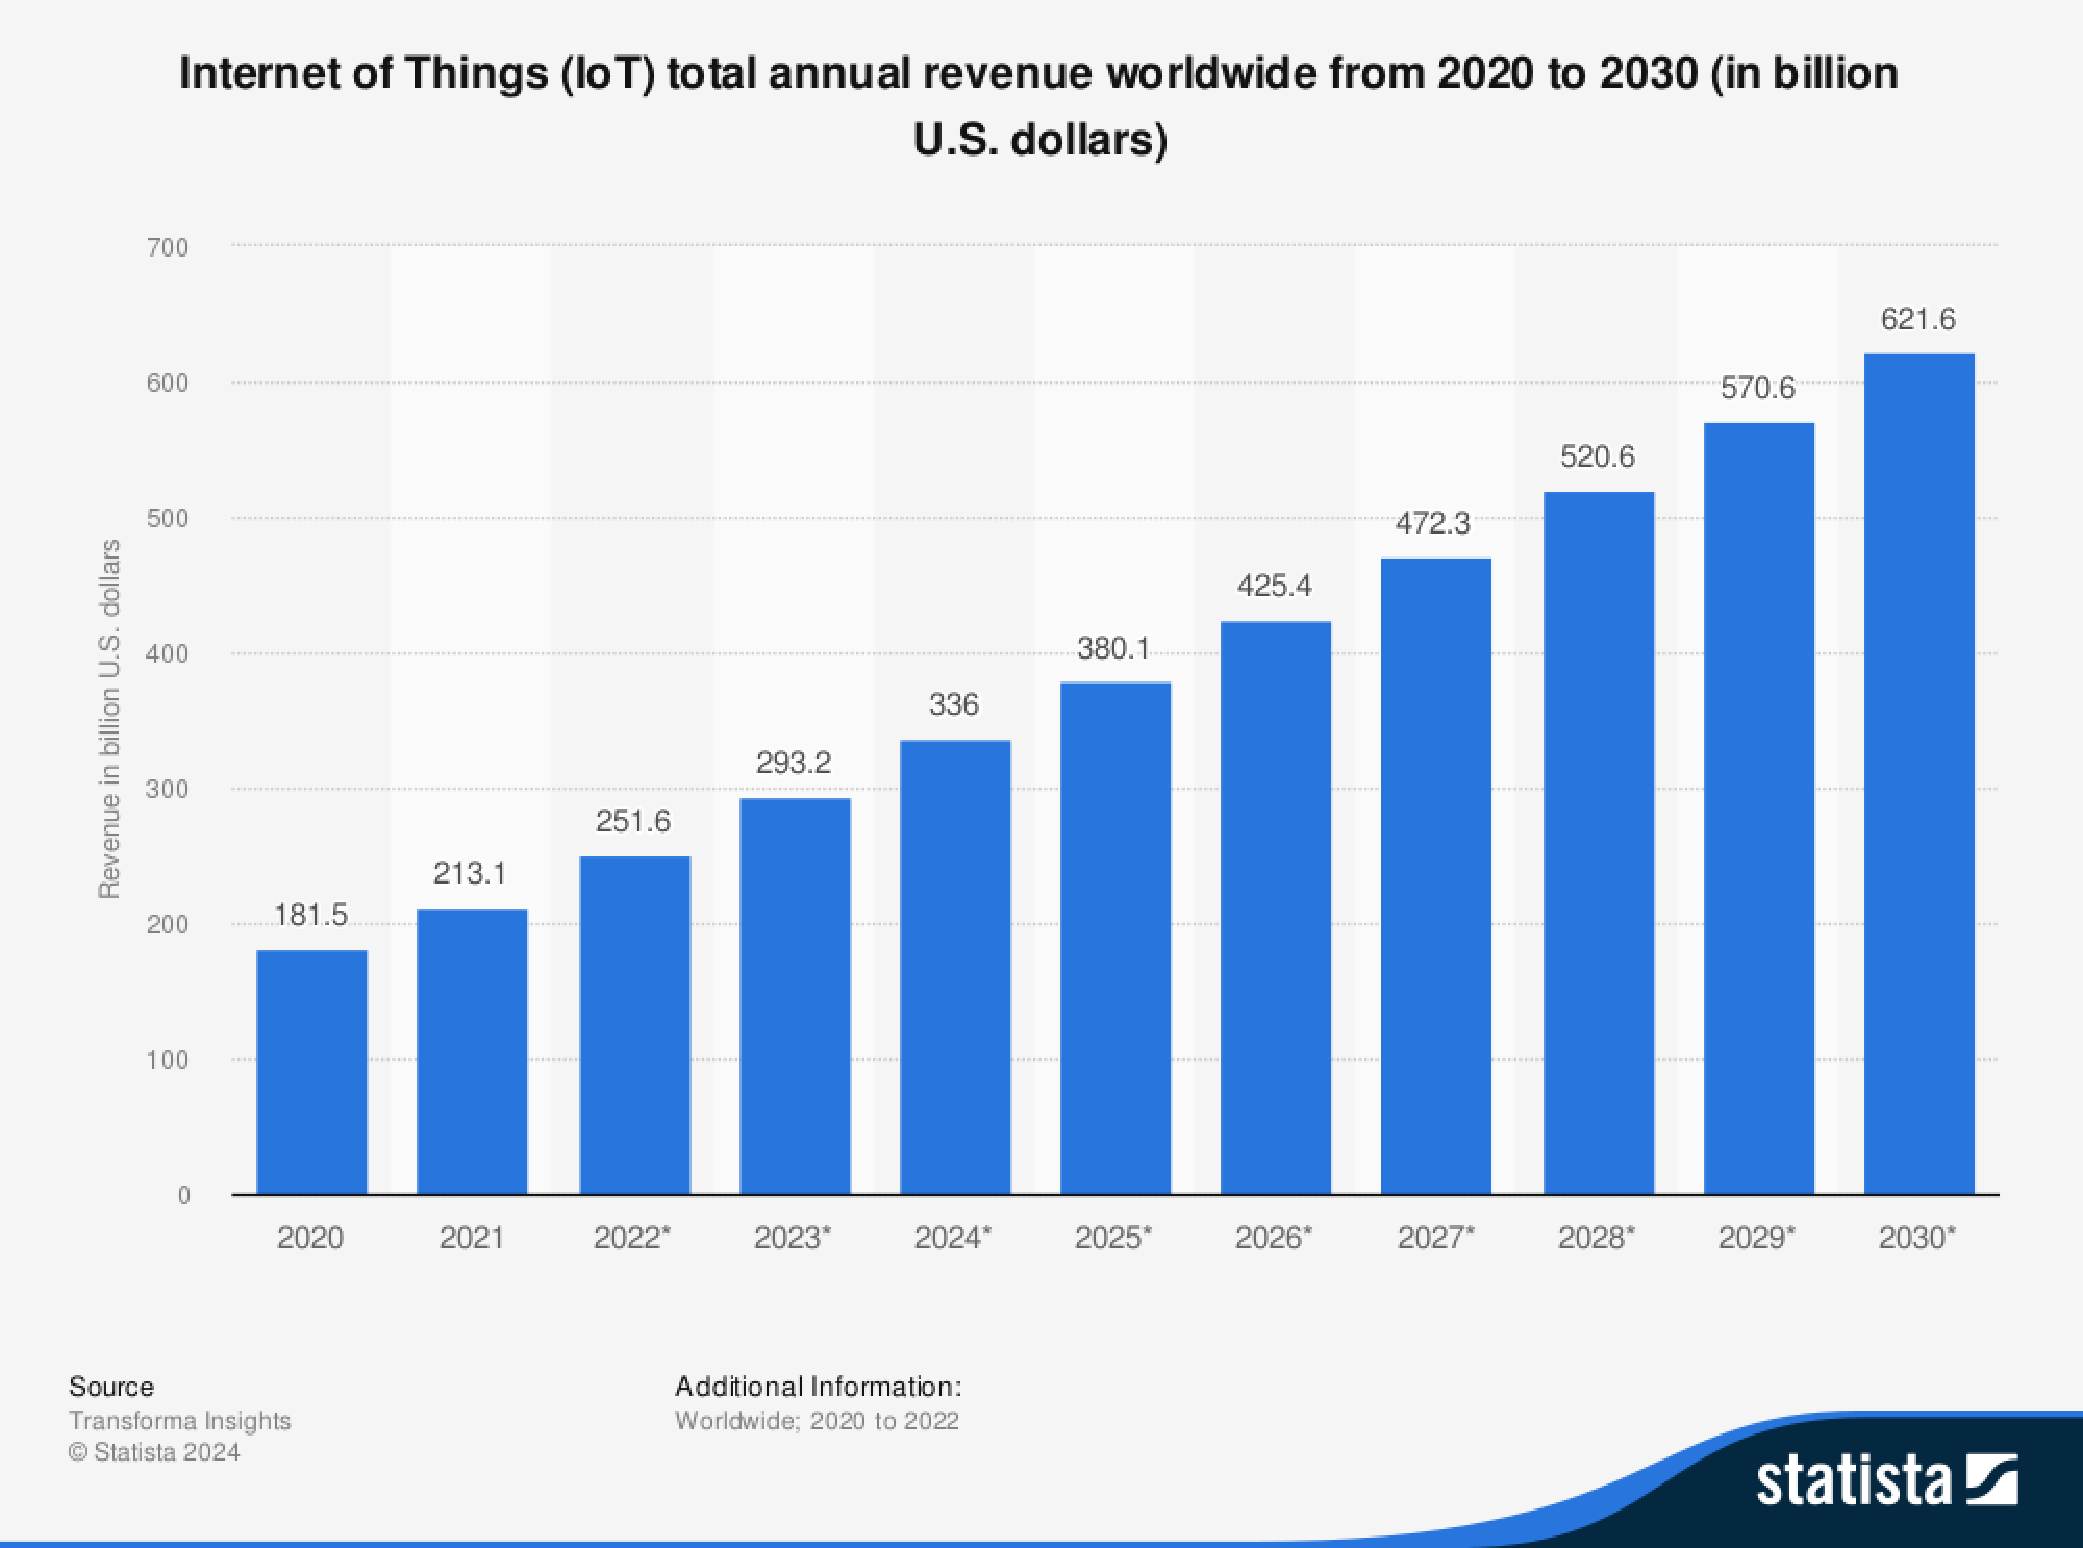
\includegraphics[width=\linewidth, trim={1.25cm 4.75cm 1cm 3.75cm}, clip]{c1_intro/img/iot_revenue.pdf}
    \caption{Internet of Things (IoT) total annual revenue worldwide from 2020 to 2030 (from~\cite{statista_iot_revenu})}
    \label{fig:iot_revenue}
\end{figure}

Embedded systems, which form the backbone of IoT devices, are particularly vulnerable to security breaches due to their limited computing resources and the need for real-time operation. These systems are frequently deployed in environments where they are exposed to potential adversaries, making them attractive targets for various types of attack. Among these, fault injection attacks have emerged as a significant threat. By deliberately introducing flaws into a system, attackers can exploit vulnerabilities to gain unauthorised access, extract sensitive information or disrupt the operation of the system.

Software security is a critical aspect of the development and deployment of software systems, encompassing measures and practices designed to protect applications from malicious attacks, vulnerabilities, and other security risks. It involves the implementation of protocols to ensure the confidentiality, integrity, and availability of software and data. This field addresses a wide range of threats, including but not limited to, code injection, buffer overflows, and unauthorized access. Effective software security practices include rigorous code reviews, the use of secure coding standards, regular vulnerability assessments, and the deployment of encryption and authentication mechanisms. As software becomes increasingly integral to various aspects of daily life and business operations, ensuring its security is paramount to safeguarding sensitive information, maintaining user trust, and preventing financial and reputational damage.

% %%%%%%%%%%%%%%%%%%%%%%%%%%%%%%%%%%%%%%%%%%%%%%%%%%%%%%%%%%%%%%%%%%%%%%%%%%%%%%%%%%%%%%%%%%%%%%%
% \section{Motivations}
attaques cyber de plus en plus répandues, nécessité de protéger les systèmes embarqués (médical, voitures, etc)
attaques physiques présentes dont les FIA
injections de fautes de plus en plus facile \cite{rayvlite_wired, rayvlite_fraktal}
nombreuses études qui montre les vulnérabilités de systèmes critiques contre les FIA (en citer 6 ou 7)


%%%%%%%%%%%%%%%%%%%%%%%%%%%%%%%%%%%%%%%%%%%%%%%%%%%%%%%%%%%%%%%%%%%%%%%%%%%%%%%%%%%%%%%%%%%%%%%
\section{Objectives}

%%%%%%%%%%%%%%%%%%%%%%%%%%%%%%%%%%%%%%%%%%%%%%%%%%%%%%%%%%%%%%%%%%%%%%%%%%%%%%%%%%%%%%%%%%%%%%%
\section{Manuscript outline}

This work is segmented in seven chapters, the first being this introduction.

Chapter~\ref{chapter:soa} presents the state of the art about Information Flow Tracking (IFT) by explaining how they work, the different types of existing IFT, this chapter presents what is physical attacks, the literature about it and presents the two principle type of physical attacks: Side-Channel Attacks and Fault Injection Attacks. Finally, the chapter presents an overview of the literature about countermeasures against Fault Injection Attacks

Chapter~\ref{chapter:dift_assessment} presents the background of this work with the presentation of the RISC-V ISA, the architecture of the D-RI5CY core and the DIFT works. Then, the use cases used in this work are going to be presented. Finally, a vulnerability assessment will be done to show how these use case are vulnerable against FIA and where.

Chapter~\ref{chapter:fissa} introduces a new tool, FISSA, to automatise fault injection campaigns in simulation. This tool allows a designer to assess his design during the conception phase. This chapter presents how it works and how to use it, and compares it to others tools available in the literature.

Chapter~\ref{chapter:countermeasures} details the different implementation of countermeasures to protect the D-RI5CY core against FIA and evaluate these protections in terms of area, performance, and efficiency.

Chapter~\ref{chapter:exp_setup_results}

Chapter~\ref{chapter:conclusion}

%%%%%%%%%%%%%%%%%%%%%%%%%%%%%%%%%%%%%%%%%%%%%%%%%%%%%%%%%%%%%%%%%%%%%%%%%%%%%%%%%%%%%%%%%%%%%%%